% Template source: University of Florida Department of Physics, https://www.phys.ufl.edu/courses/phy4803L/sample-paper.zip

\documentclass[aps,twocolumn,secnumarabic,nobalancelastpage,amsmath,amssymb,nofootinbib,floatfix,letterpaper]{revtex4}

% Documentclass Options
    % aps, prl, rmp stand for American Physical Society, Physical Review Letters, and Reviews of Modern Physics, respectively
    % twocolumn permits two columns, of course
    % nobalancelastpage doesn't attempt to equalize the lengths of the two columns on the last page
        % as might be desired in a journal where articles follow one another closely
    % amsmath and amssymb are necessary for the subequations environment among others
    % secnumarabic identifies sections by number to aid electronic review and commentary.
    % nofootinbib forces footnotes to occur on the page where they are first referenced
        % and not in the bibliography
    % REVTeX 4 is a set of macro packages designed to be used with LaTeX 2e.
        % REVTeX is well-suited for preparing manuscripts for submission to APS journals.


\usepackage{chapterbib}    % allows a bibliography for each chapter (each labguide has it's own)
\usepackage{color}         % produces boxes or entire pages with colored backgrounds
\usepackage{graphics}      % standard graphics specifications
\usepackage[pdftex]{graphicx}      % alternative graphics specifications
\usepackage{epsf}          % old package handles encapsulated post script issues
\usepackage{bm}            % special 'bold-math' package
\usepackage{verbatim}			% for comment environment
\usepackage[colorlinks=true,citecolor=blue]{hyperref}  % this package should be added after all others
                                        % use as follows: \url{https://urldefense.proofpoint.com/v2/url?u=http-3A__web.mit.edu_8.13&d=DwICAg&c=sJ6xIWYx-zLMB3EPkvcnVg&r=D88uS55Tats-jlFQAC1XryFUYq8B7Lk3StFbXzgsiB4&m=Vjrc9Wj5n5rkIDMPJ5VsRj2GyXC3yXmN_zDHey6dVio&s=_byqsJfgO464rVIugNWFPmbBeIYfNiJcGS1fgIwc0m4&e= }

\usepackage{subcaption}
\usepackage{float}
\usepackage{siunitx}
\usepackage{textcomp}
\usepackage{gensymb}
\usepackage{tikz}
\usepackage{multirow}
\usepackage{xcolor}
\usepackage{circledsteps}

\usepackage{natbib}
\bibliographystyle{ieeetr}
\def\bibsection{\section{References}} 

% Graph stuff
\usepackage[utf8]{inputenc}
\usepackage{pgfplots}
\usepgfplotslibrary{groupplots,dateplot}
\usetikzlibrary{patterns,shapes.arrows}
\pgfplotsset{compat=newest}
\usepackage{shellesc}
\usetikzlibrary{external}
\tikzexternalize

% Define colours
\definecolor{darkgreen}{HTML}{228833}

\usepackage[english]{babel}
\usepackage[autostyle, english=american]{csquotes}
\MakeOuterQuote{"}

\renewcommand{\thetable}{\arabic{table}}

\begin{document}
\title{Investigating the Accuracy of the Damped Simple Pendulum Model}
\author{Tyler Tian}
\noaffiliation
\date{\today}


% \begin{abstract}
% \end{abstract}

\maketitle

%%%%%%%%%%%%%%%%%%%%%%%%%%%%%%%%%%%%%%%%%%%%%%%%%%%%%%%%%%%%%%%%%%

\section{Introduction}

This lab report aims to quantitatively evaluate how well the theoretical model for a damped simple pendulum actually
performs in reality.

Pendulums are one of the classic textbook examples of a damped harmonic oscillator. Most physics students will be able
to tell you that for small angles, the motion of an idealized pendulum can be modelled by
\begin{equation}
    \theta(t) = \theta_0 e^{-\frac{t}{\tau}}\cos\left(2\pi\frac{t}{T} + \phi_0\right)
    \label{eqn:model}
\end{equation}
where \(\theta(t)\) is the angle of the pendulum in radians at time \(t\), \(\theta_0\) is the initial amplitude at
release, \(\tau\) is the time constant of decay, \(T\) is the period and \(\phi_0\) is the phase shift \cite{lab}.

This model carries some assumptions, such as a frictionless pivot, massless string, a damping force
proportional to velocity, and the small angle approximation \(\sin \theta \approx \theta\). While they make the
the model simple to use, these idealized conditions are clearly not true in real life.

To what extent, then, is this a good approximation of a real pendulum? To scientifically investigate this question, a
pendulum with an adjustable string length and bob mass is constructed (Figure \ref{fig:swingy}), and a series of
experiments were performed on it to evaluate its agreement with the theoretical model.

\begin{figure}[htb]
    \centering
    \includegraphics[width=0.6\linewidth]{swingy.jpg}
    \caption{Swingy the pendulum.}
    \label{fig:swingy}
\end{figure}

3 Labs were performed according to the Lab handout \cite{lab}. An overview of the procedure and result is given for each
Lab below:
\begin{enumerate}
    \item
    \textbf{Lab 1: \(Q\) Factor:}
    The \(Q\) factor is a property of the pendulum that measures the rate of decay \cite{lab}. It is defined by:
    \begin{equation}
        Q = \pi\frac{\tau}{T}
        \label{eqn:qfactor}
    \end{equation}

    In this Lab, the \(Q\) factor is measured using two independent methods described in Section \ref{sec:lab1_method}.
    The fitting method produces a \(Q\) of \(142 \pm 4\) and the oscillation counting method produces a \(Q\) of
    \(148 \pm 2\). The values are found to be mostly consistent. However, the fit of the data to Equation \ref{eqn:model}
    leads to the conclusion that the model is not an accurate predictor of the pendulum's long-term behaviour.

    \item
    \textbf{Lab 2: Period vs. Amplitude:}
    This Lab investigates the relationship between period and amplitude by fitting a power series to the data (Section
    \ref{sec:lab2_method}).
    According to Equation \ref{eqn:model}, the period should be constant, but a quadratic relationship between period and
    amplitude is found for large amplitudes (Section \ref{sec:lab2_relationship}).

    \item
    \textbf{Lab 3: Period vs. String Length and Mass:}
    Part a of this lab investigates the relationship between period and string length and compares it to the theoretical
    model of \(T \approx 2\sqrt{L}\) \cite{lab} by fitting an equation to the data (Section \ref{sec:lab3_method}).
    The theoretical model is found to be a good approximation of the actual behaviour, although the exact values
    produced by the fit are not quite in agreement with the theoretical values (Section \ref{sec:lab3a_analysis}).

    Part b of this lab investigates the relationship between period and mass. According to Equation \ref{eqn:model},
    mass should not have a direct effect on period, and the data is found to agree with this (Section
    \ref{sec:lab3b_analysis}).
\end{enumerate}

The results confirm the hypothesis that Equation \ref{eqn:model} only works for small angles. The real behaviour begins to
deviate from the model for amplitudes greater than \(17.2\degree\) and deviates appreciably when the amplitude is
greater than \(45\degree\).

In terms of time range, the model is a good approximation of the short-term behaviour of the system (such as period)
for small angles, but not a good approximation of the long-term behaviour. Notably, the model's rate of decay is
significantly faster than the real rate of decay, and also accumulates a phase offset if the starting angle is large
since it does not take into account changes in period.

%%%%%%%%%%%%%%%%%%%%%%%%%%%%%%%%%%%%%%%%%%%%%%%%%%%%%%%%%%%%%%%%%%

\section{Method}

\subsection{Pendulum Construction}

\begin{figure}[htb]
    \centering
    \begin{subfigure}{\linewidth}
        \includegraphics[width=0.7\linewidth]{pivot.jpg}
        \caption{The pivot mechanism.}
        \label{fig:pivot}
    \end{subfigure}
    \begin{subfigure}[t]{0.49\linewidth}
        \includegraphics[height=0.65\linewidth]{clip.jpg}
        \caption{Binder clip to hold the string and measuring tape to measures change in string length.}
        \label{fig:clip}
    \end{subfigure}
    \begin{subfigure}[t]{0.49\linewidth}
        \includegraphics[height=0.65\linewidth]{cup.jpg}
        \caption{Red cup with coins inside for weight. Note the braided string used here.}
        \label{fig:cup}
    \end{subfigure}
    \caption{Features of the pendulum.}
\end{figure}

The main support structure of the pendulum consists of two pieces of wood attached with screws.
This was chosen because the material was readily available, and could be substituted for any material of
similar size and suitable strength.

The pendulum uses a thin, braided string, specifically chosen to minimize twisting in order to prevent the bob from
spinning. The string is lightly wound around a nail, and then directed through a hole in the support board and held
in place by a binder clip (Figure \ref{fig:pivot}). A flat measuring tape is secured parallel to the string to measure
changes in the string length (Figure \ref{fig:clip}). A piece of green masking tape is put over the pivot nail to enable
computer-vision based tracking.

The string is attached to a bob consisting of a small, red plastic cup, specifically chosen for its high colour contrast
against the background to enable precise vision tracking. The cup is loaded with coins to vary its weight since coins
have known masses (Figure \ref{fig:cup}).

\subsection{Pendulum Tracking}
\label{sec:tracking}

\begin{figure}[htb]
    \centering
    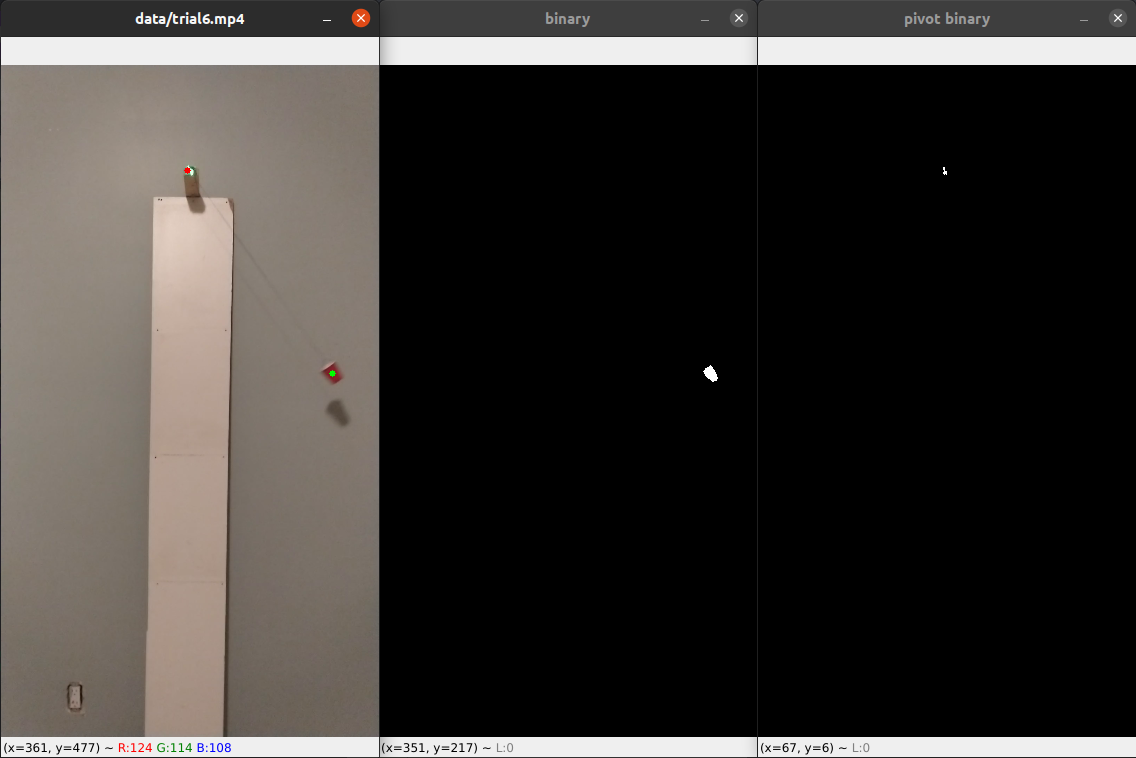
\includegraphics[width=\linewidth]{cv_track.png}
    \caption{CV-based tracking of the pendulum.}
    \label{fig:tracking}
\end{figure}

Videos of the pendulum are shot on a phone camera and then passed to a Python program written with OpenCV (see Appendix
\ref{appendix:code}). The locations of the bob and pivot are determined by thresholding the image in the HSV colour
space (the right two windows in Figure \ref{fig:tracking}), and then taking the average of the pixels that passed the
threshold to obtain the centres of the bob and pivot in the image (green and red dots in the first window in Figure
\ref{fig:tracking}). After the pixel coordinates have been determined, the ratio of the difference between the \(x\) and
\(y\) coordinates are used to compute the angle for each frame.

\subsection{Lab 1: \texorpdfstring{\(Q\)}{Q} Factor}
\label{sec:lab1_method}

For this Lab, the video is shot at 60fps but only sampled at 30Hz since precise measurements are less important for
determining the \(Q\) factor. Subsequent experiments have improved this.

The string length is fixed at approximately 65cm and the mass at approximately 42g. The precise masses and lengths are
never measured as they remained constant and are unimportant for this Lab.

The \(Q\) factor is obtained from the angle-time data using two independent methods:
\begin{enumerate}
    \item
        \textbf{Curve fitting:} A Python program (see Appendix \ref{appendix:code}) is used to fit the model (Equation
        \ref{eqn:model}) to the data, producing values for \(\tau\) and \(T\). \(Q\) is calculated from these values
        using Equation \ref{eqn:qfactor}.
    \item
        \textbf{Oscillation counting:} By substituting \(t = T\frac{Q}{n}\) (i.e. \(\frac{Q}{n}\) oscillations) into
        the decay term in Equation \ref{eqn:model}, the term becomes
        \begin{equation}
            \theta_0 e^{-\frac{T\frac{Q}{n}}{\tau}} = \theta_0 e^{-\frac{T\frac{\pi\frac{\tau}{T}}{n}}{\tau}} = \theta_0 e^{-\frac{\pi}{n}}
        \end{equation}
        which shows that \(\frac{Q}{n}\) can be measured by counting the number of oscillations of the pendulum until
        its amplitude decays to a factor of \(e^{-\frac{\pi}{n}}\) times the initial amplitude at release.
        
        A Python program (see Appendix \ref{appendix:code}) is used to count these oscillations. Half-oscillations are
        counted as the pendulum swings from a positive peak to a negative peak. For example, if the pendulum starts on
        the right, but first reaches the target amplitude when it is swinging to the left, then a half-oscillation will
        be counted for the last cycle. \(\frac{Q}{3}\) is measured for this Lab because not enough oscillations were
        recorded to measure for \(\frac{Q}{2}\) or \(Q\) directly.

        For both parts, only small release angles are used so the effect of decaying amplitude on period is negligible.
\end{enumerate}

\subsection{Lab 2: Relationship Between Period and Amplitude}
\label{sec:lab2_method}

For this Lab, the video is shot at 120fps to reduce motion blur caused by the increased speeds of the bob, but the video
is still sampled at 30Hz. The string length and bob mass are the same as Lab 1 (Section \ref{sec:lab1_method}).

To convert from raw time-angle data to amplitude-period data required for this Lab, a Python program was used to find
the peaks and valleys of the graph, as shown in Figure \ref{fig:rawdata} (see Appendix \ref{appendix:code}).
Since the data was somewhat noisy, multiple peak points were averaged to find the time of each peak, and the
maximum/minimum of these peak points were taken to find the peak amplitude.

\begin{figure}[htb]
    \begin{tikzpicture}
        \begin{axis}[
            title=Angle vs. Time,
            xlabel=Time (s),
            ylabel=Angle (rad),
            legend entries={Raw Data, Min/Max}
        ]
            \addplot+[
                only marks,
                mark size=1pt,
            ] table [x index=0, y index=1] {trial1_rawdata.txt};
            \addplot+[
                only marks,
                mark size=1.5pt,
            ] table [x index=0, y index=1] {trial1_extrema.txt};
        \end{axis}
    \end{tikzpicture}
    \caption{Zoomed-in view of the first 500 raw data points with the peaks marked.}
    \label{fig:rawdata}
\end{figure}

Measuring the period by taking the time for multiple oscillations and dividing by the number of oscillations will reduce
the period uncertainty, but increase the amplitude uncertainty as the amplitude decays more over a longer period of
time. Conversely, taking the time for half an oscillation and then multiplying by 2 increases the period uncertainty but
reduces the amplitude uncertainty as there is now less decay. Because the \(Q\) factor as determined in Lab 1 (Section
\ref{sec:lab1_analysis}) is reasonably but not extremely large, the period is measured directly using the difference in
time between adjacent peaks, without averaging over multiple oscillations or looking at half an oscillation.

After the period-amplitude data has been collected, a power series is fit to the data using a Python program
(Appendix \ref{appendix:code}) using least-squares regression:
\begin{equation}
    T(\theta) = T_0 + B\theta + C\theta^2 + D\theta^3 + \cdots
    \label{eqn:power_series}
\end{equation}

Since Equation \ref{eqn:power_series} contains an infinite number of terms, it cannot be used directly in the fit, so it
is truncated to produce 5 polynomials of degrees 0-4 respectively, and a fit is done separately for each.

\subsection{Lab 3: Relationship Between Period and Length/Mass}
\label{sec:lab3_method}

For this Lab, the video was shot at 30fps and sampled at 30Hz. As determined in Lab 2 (Section \ref{sec:lab2_relationship}),
this does have an impact on period, but this effect can be ignored for sufficiently small angles. Therefore the release
angle of the pendulum in this Lab is always less than the constraint determined in Section \ref{sec:lab2_range}.
As the effect of decaying period is now negligible, multiple (about 10 each) oscillations were measured for every
length/mass.

The period produced by each length/mass is determined using the same method as outlined in Section
\ref{sec:lab2_method}, with yet another Python program (see Appendix \ref{appendix:code}).

\subsubsection{Lab 3a: Period vs. Length}

To determine the effective string length, the bob is raised to the top as shown in Figure \ref{fig:raised_bob}, and a
reading is taken on the measuring tape shown in the left of Figure \ref{fig:swingy} and used as a base value. For
every trial, a reading is taken and subtracted from this base value to determine the added length.

\begin{figure}[htb]
    \includegraphics[width=0.7\linewidth]{bob_top.jpg}
    \caption{Reducing the string length to the shortest possible.}
    \label{fig:raised_bob}
\end{figure}

To determine the remaining length between the pivot and the bob's centre of mass in Figure \ref{fig:raised_bob}, a
measuring tape is used. Since the cup is much lighter than the coins inside, the centre of mass is estimated to be the
centre of mass of the 6 coins inside. The distance between the top of the 3rd coin and the pivot is measured and added
to each length to determine the final effective length.

Once the data is collected, the following function is fit to it using a Python program (see Appendix \ref{appendix:code})
using ODR (Orthogonal Distance Regression):
\begin{equation}
    T(L) = k(L_0 + L)^n
    \label{eqn:period}
\end{equation}

Finally, the fit parameters produced are compared with their theoretical values discussed in Section \ref{sec:lab3a_results}.

\subsubsection{Lab 3b: Period vs. Mass}

To determine the bob's mass, the cup's mass is measured on a digital scale. Due to the activity being completed at home,
high-precision scales are often unavailable, so the mass of the coins inside is calculated using masses according to the
Royal Canadian Mint \cite{mint}.

As the coins are loaded into the cup, the centre of mass may shift and change the effective string length, which affects
the period. To reduce this uncertainty, a long string length was used so that the effect of any shift is minimized.

The increased mass of the coins may also stretch the string and increase the string length. To correct for this error,
the amount the string stretches for each mass is determined using a measured spring constant. The new length is put back
into Equation \ref{eqn:period}, and an estimate of the difference in period caused by stretching is calculated. This
correction is then subtracted from each period. This process is discussed in more detail in Section
\ref{sec:lab3b_correction}.

%%%%%%%%%%%%%%%%%%%%%%%%%%%%%%%%%%%%%%%%%%%%%%%%%%%%%%%%%%%%%%%%%%

\section{Lab 1 Results and Analysis}

\subsection{Uncertainties}
\label{sec:lab1_uncert}

There are two sources of measurement uncertainty during the data collection process shared by both methods:
\begin{enumerate}
    \item 
        \textbf{Time measurement uncertainty from the camera's frame rate and shutter speed.} Because the camera only
        captures a set number of frames per second, this creates a small uncertainty about the exact time that data
        points occurred. An upper bound for this uncertainty can be obtained by taking the time between two frames and
        dividing by 2. For a 60fps video, this results in an uncertainty of \(\pm 0.008\si{s}\).
    \item
        \textbf{Angle measurement uncertainty from motion blur and imperfect tracking.} Motion blur caused by a
        fast-moving bob can make the angle hard to measure, and imperfect computer vision tracking of the bob and
        pivot may also result in an incorrect angle. To estimate an upper bound of this uncertainty, a frame is taken
        from when the pendulum has its maximum velocity to maximize motion blur. Two lines are drawn representing the
        worst possible cases for tracking (Figure \ref{fig:angle_uncert}), and the angle between them is taken. The
        result is a range of about \(5\degree\), or an uncertainty of \(\pm 3\degree\)/\(\pm 0.05\si{rad}\).
        
        (Note: Further analysis of the behaviour of the tracking program shows this to be an overly conservative
        estimate, since the averaging of the pixel coordinates as described in Section \ref{sec:tracking} produces the
        centre of the bob reliably even when there is motion blur. Thus, while this uncertainty is shown in the later
        graphs, it is not used in the final analysis.)
\end{enumerate}
\begin{figure}[htb]
    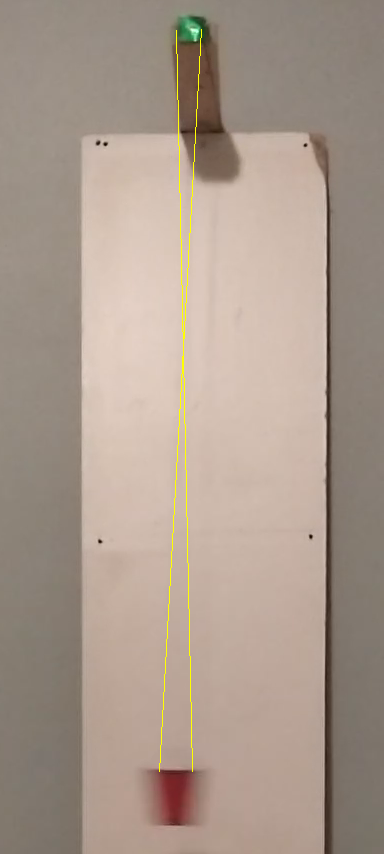
\includegraphics[width=0.3\linewidth]{uncert1.png}
    \caption{Worst-case scenarios for angle uncertainty. Blue lines are drawn to indicate the greatest and least
        possible angle. Note that this is a very conservative estimate.}
    \label{fig:angle_uncert}
\end{figure}

These uncertainties are shown in the graphs in Figure \ref{fig:lab1_fitzoom}. They are very small when
compared to the uncertainties later in the experiment, and so they will be ignored as only the largest uncertainty is
considered for this Lab.

There are also other sources of measurement uncertainty that are much harder to quantify, such as perspective
distortion and camera tilt. These uncertainties are assumed to be smaller and random, and thus incorporated in other
sources.

Specifically for method 1 (curve fitting), the least-squares fit generates a covariance matrix, which contains the
standard deviations of each fit parameters. These standard deviations are used as the uncertainties for \(\tau\) and
\(T\), and propagated to \(Q\) by taking the largest relative uncertainty.

Specifically for method 2 (oscillation counting), amplitude can only be determined at a positive or negative peak, which
gives the oscillation count a maximum resolution of 0.5 (Section \ref{sec:lab1_method}). When multiplied by 3 to find
\(Q\), this represents an uncertainty of \(\pm 1.5\).

For both methods, 7 trials were conducted, and the uncertainty of the mean of these trials is used as another source of
uncertainty.

\subsection{Results from Curve Fitting}

\begin{figure*}[t]
    \centering
    \begin{subfigure}{\textwidth}
        \begin{tikzpicture}
            \begin{axis} [
                title=Best Fit Curve,
                xlabel=Time (s),
                ylabel=Angle (rad),
                width=\textwidth,
                height=0.2\textheight,
                xmin=-3,
                xmax=120,
                extra y ticks={0},
                extra y tick labels={},
                extra y tick style={grid=major},
                clip marker paths=true,
                legend entries={Collected Data, Best Fit Curve}
            ]
                \addplot+[
                    only marks,
                    mark size=1pt,
                ] table [
                    x index=0,
                    y index=1,
                ] {lab1_data.txt};
                \addplot [
                    thick,
                    red,
                    domain=0:117,
                    samples=2000,
                ] {0.6057992432358721 * e ^ (-x / 80.4722570265344) * cos(deg(2 * pi * x / 1.6499108861456369 - 0.6356025015941729))};
            \end{axis}
        \end{tikzpicture}
        \begin{tikzpicture}
            \begin{axis} [
                title=Fit Residuals,
                xlabel=Time (s),
                ylabel=Angle (rad),
                width=\textwidth,
                height=0.2\textheight,
                xmin=-3,
                xmax=120,
                extra y ticks={0},
                extra y tick labels={},
                extra y tick style={grid=major},
            ]
                \addplot+[
                    only marks,
                    mark size=1pt
                ] table [
                    x index=0,
                    y index=2,
                ] {lab1_data.txt};
            \end{axis}
        \end{tikzpicture}
        \caption{Result of fitting Equation \ref{eqn:model} to one of the trials. For this particular fit, \(A = 0.606\),
            \(\tau = 80.5\), \(T = 1.65\), \(\phi = -0.636\). Uncertainty bars are omitted to improve readability.}
        \label{fig:lab1_fit}
    \end{subfigure}
    \begin{subfigure}{\textwidth}
        \begin{tikzpicture}
            \begin{axis} [
                title=Best Fit Curve,
                xlabel=Time (s),
                ylabel=Angle (rad),
                width=\textwidth,
                height=0.2\textheight,
                xmin=-0.5,
                xmax=10.5,
                extra y ticks={0},
                extra y tick labels={},
                extra y tick style={grid=major},
                clip marker paths=true,
                legend entries={Collected Data, Best Fit Curve}
            ]
                \addplot+[
                    only marks,
                    mark size=1pt,
                    restrict expr to domain={x}{0:10},
                    error bars/.cd,
                        x dir=both,
                        y dir=both,
                        x explicit,
                        y explicit,
                        x fixed=0.008,
                        y fixed=0.05,
                ] table [
                    x index=0,
                    y index=1,
                ] {lab1_data.txt};
                \addplot [
                    thick,
                    red,
                    domain=0:10,
                    samples=200,
                ] {0.6057992432358721 * e ^ (-x / 80.4722570265344) * cos(deg(2 * pi * x / 1.6499108861456369 - 0.6356025015941729))};
            \end{axis}
        \end{tikzpicture}
        \begin{tikzpicture}
            \begin{axis} [
                title=Fit Residuals,
                xlabel=Time (s),
                ylabel=Angle (rad),
                width=\textwidth,
                height=0.2\textheight,
                xmin=-0.5,
                xmax=10.5,
                extra y ticks={0},
                extra y tick labels={},
                extra y tick style={grid=major},
            ]
                \addplot+[
                    only marks,
                    mark size=1pt,
                    restrict expr to domain={x}{0:10},
                    error bars/.cd,
                        x dir=both,
                        y dir=both,
                        x explicit,
                        y explicit,
                        x fixed=0.008,
                        y fixed=0.05,
                ] table [
                    x index=0,
                    y index=2,
                ] {lab1_data.txt};
            \end{axis}
        \end{tikzpicture}
        \caption{Zoomed-in view of the first 15 seconds of the data, showing the uncertainties. Note the significant
            deviation of the best-fit curve from the actual data.}
        \label{fig:lab1_fitzoom}
    \end{subfigure}
    \caption{Fitting Equation \ref{eqn:model} to data from one of the trials.}
    \label{fig:lab1_graph}
\end{figure*}

Figure \ref{fig:lab1_graph} shows the result of fitting Equation \ref{eqn:model} for one of the trials.
\(Q\) values computed using this method are shown in Table \ref{table:lab1_fit}.

\begin{table}[ht]
    \begin{tabular}{c|c|c|c}
        Trial & \(Q\) & Uncertainty & \% Uncertainty \\
        \hline
        1   & 153.23    & \(\pm 3.65\) & 2.38 \\
        2   & 147.89    & \(\pm 3.95\) & 2.67 \\
        3	& 140.96	& \(\pm 3.53\) & 2.51 \\
        4	& 151.12	& \(\pm 3.81\) & 2.52 \\
        5	& 130.24	& \(\pm 3.86\) & 2.96 \\
        6	& 131.31	& \(\pm 3.76\) & 2.86 \\
        7	& 138.04	& \(\pm 3.70\) & 2.68 \\
        \hline
        \multicolumn{3}{l}{Mean} & 141.83 \\
        \multicolumn{3}{l}{Standard Deviation} & 9.24 \\
        \multicolumn{3}{l}{Uncertainty of the Mean} & 3.49
    \end{tabular}
    \caption{Raw data from curve fitting; values are unrounded.}
    \label{table:lab1_fit}
\end{table}

From Table \ref{table:lab1_fit}, the greatest percentage uncertainty is trial 5 with an uncertainty of 2.96\%. When
multiplied by the mean, this corresponds to an uncertainty of \(\pm 4.20\), which is greater than the uncertainty of
the mean. \textbf{The final value as determined by this method is \(Q = 142 \pm 4\).}

\subsection{Results from Oscillation Counting}

\(Q\) values computed using this method are shown in Table \ref{table:lab1_osc}.

\begin{table}[ht]
    \begin{tabular}{c|c|c|c}
        Trial & \(Q\) & Uncertainty & \% Uncertainty \\
        \hline
        1   & 148.5 & \(\pm 1.5\) & 1.01 \\
        2   & 151.5 & \(\pm 1.5\) & 0.99 \\
        3	& 148.5 & \(\pm 1.5\) & 1.01 \\
        4	& 154.5 & \(\pm 1.5\) & 0.97 \\
        5	& 139.5 & \(\pm 1.5\) & 1.08 \\
        6	& 142.5 & \(\pm 1.5\) & 1.05 \\
        7	& 148.5 & \(\pm 1.5\) & 1.01 \\
        \hline
        \multicolumn{3}{l}{Mean} & 147.6 \\
        \multicolumn{3}{l}{Standard Deviation} & 5.11 \\
        \multicolumn{3}{l}{Uncertainty of the Mean} & 1.93
    \end{tabular}
    \caption{Raw data from oscillation counting; values are unrounded.}
    \label{table:lab1_osc}
\end{table}

From Table \ref{table:lab1_osc}, the greatest percentage uncertainty is trial 5 with an uncertainty of 1.08\%, which
corresponds to an uncertainty of \(\pm 1.59\) in \(Q\), less than the uncertainty of the mean. \textbf{The final value
as determined by this method is \(Q = 148 \pm 2\).}

However, an interesting phenomenon can be observed by varying the fraction of \(Q\) to measure for.
For example, by measuring for \(\frac{Q}{4}\) instead, the data in Table \ref{table:lab1_osc4} is obtained, which has a
significantly different mean \(Q\) value.

\begin{table}[ht]
    \begin{tabular}{c|c|c|c}
        Trial & \(Q\) & Uncertainty & \% Uncertainty \\
        \hline
        1   & 126.0 & \(\pm 2\) & 1.59 \\
        2   & 138.0 & \(\pm 2\) & 1.45 \\
        3	& 134.0 & \(\pm 2\) & 1.49 \\
        4	& 144.0 & \(\pm 2\) & 1.39 \\
        5	& 128.0 & \(\pm 2\) & 1.56 \\
        6	& 126.0 & \(\pm 2\) & 1.59 \\
        7	& 134.0 & \(\pm 2\) & 1.49 \\
        \hline
        \multicolumn{3}{l}{Mean} & 132.9 \\
        \multicolumn{3}{l}{Standard Deviation} & 6.72 \\
        \multicolumn{3}{l}{Uncertainty of the Mean} & 2.54
    \end{tabular}
    \caption{Data obtained from measuring \(\frac{Q}{4}\) instead; values are unrounded. Note how the mean
        \(Q\) value deviates significantly from the one obtained in Table \ref{table:lab1_osc}.}
    \label{table:lab1_osc4}
\end{table}

After more trials, it was observed that the value of \(Q\) obtained through counting oscillations is dependent on the
fraction of \(Q\) that was counted for. Moreover, as the denominator increases, the observed \(Q\) value seems to
decrease. This is not in agreement with the model since according to Equations \ref{eqn:model} and \ref{eqn:qfactor}
\(Q\) should be independent of the fraction measured.

\subsection{Discussion and Analysis}
\label{sec:lab1_analysis}

\subsubsection{\texorpdfstring{\(Q\)}{Q} Factor}
\label{sec:lab1_qfactor}

The \(Q\) value obtained by oscillation counting is within 1.5 times the uncertainty of the \(Q\) value obtained by
curve fitting. If values follow a normal distribution, there is a 13.4\% chance for values to be more than 1.5 times the
uncertainty away. From this we conclude that \textbf{while there is a discrepancy between the two \(Q\) values, the
values could be in agreement.}

However, as shown in Table \ref{table:lab1_osc4}, by measuring for \(\frac{Q}{4}\) a \(Q\) value of \(133 \pm 3\) is
obtained instead. This value is 2.25 times the uncertainty away from the \(Q\) value obtained by curve fitting, and 5
times the uncertainty away from the \(Q\) value obtained by counting for \(\frac{Q}{3}\), which clearly disagrees with
either \(Q\) value found above.

Furthermore, as the fraction of \(Q\) measured for gets smaller, the measured \(Q\) value gets even further from the
values obtained previously. It can be concluded that, at least for this particular pendulum, \textbf{oscillation
counting is not a reliable way for obtaining \(Q\)}. As a result, the final \(Q\) value is taken to be the one obtained
through curve fitting (\(Q = 142 \pm 4\)).

\subsubsection{Model Accuracy}
\label{sec:lab1_accuracy}

\begin{figure*}[t]
    \begin{tikzpicture}
        \begin{axis} [
            title=Best Fit Curve,
            xlabel=Time (s),
            ylabel=Angle (rad),
            width=\textwidth,
            height=0.2\textheight,
            xmin=-3,
            xmax=120,
            extra y ticks={0},
            extra y tick labels={},
            extra y tick style={grid=major},
            clip marker paths=true,
            legend entries={Collected Data, Best Fit Curve}
        ]
            \addplot+[
                only marks,
                mark size=1pt,
            ] table [
                x index=0,
                y index=1,
            ] {lab1_data2.txt};
            \addplot [
                thick,
                red,
                domain=0:117,
                samples=2000,
            ] {0.663973140409552 * e ^ (-x / 55.2123562331802) * cos(deg(2 * pi * x / 1.656087056926946))};
        \end{axis}
    \end{tikzpicture}
    \begin{tikzpicture}
        \begin{axis} [
            title=Fit Residuals,
            xlabel=Time (s),
            ylabel=Angle (rad),
            width=\textwidth,
            height=0.2\textheight,
            xmin=-3,
            xmax=120,
            extra y ticks={0},
            extra y tick labels={},
            extra y tick style={grid=major},
        ]
            \addplot+[
                only marks,
                mark size=1pt
            ] table [
                x index=0,
                y index=2,
            ] {lab1_data2.txt};
        \end{axis}
    \end{tikzpicture}
    \caption{Result of fitting to the same data but with \(\phi_0 = 0\) (Equation \ref{eqn:model_nophi}). For this
        particular fit, \(A = 0.664\), \(\tau = 55.2\), \(T = 1.66\). Uncertainty bars are omitted to improve readability.}
    \label{fig:lab1_fit2}
\end{figure*}

An inspection of the residuals in Figure \ref{fig:lab1_graph} shows a clear pattern, which would not be present if the fit
represents the data well. At many points, the residuals reach a value of 0.2, which is over 25\% of the actual
amplitude of the data, 0.8. The amplitude of the fit also deviates significantly from the actual amplitude of the data
(0.6 versus 0.8), but adjusting the conditions of the fit does not improve it. The fit also seems to deviate
significantly from the actual data near the beginning and end of the data set as shown in Figure \ref{fig:lab1_fitzoom}.

The two possible reasons for this happening are either that the fit was not done well, or the model does not reflect the
real data well. The data is inconclusive for determining which is the dominant effect for sure, but there is evidence to
suggest that the model may not be entirely accurate.

Since time \(t = 0\) is taken to be when the pendulum is first released, the theoretical value of \(\phi_0\) should
always be 0, so the model is reduced to
\begin{equation}
    \theta(t) = \theta_0 e^{-\frac{t}{\tau}}\cos\left(2\pi\frac{t}{T}\right)
    \label{eqn:model_nophi}
\end{equation}

However, all the trials produce nonzero values for \(\phi_0\). The result of fitting to the same data but with
\(\phi_0\) removed is shown in Figure \ref{fig:lab1_fit2}. Compared to Figure \ref{fig:lab1_fit}, this time the fit is
much worse, with the fit curve deviating significantly from the data in both magnitude and phase near the end, where
visually the fit seems to be off by more than \(\frac{1}{4}\) of a period. The residuals seem to keep on increasing at
the end and are much larger than the uncertainties, which shows that \textbf{Equation \ref{eqn:model} is not an
accurate model of this pendulum for large values of \(t\)}.

This might be because Equation \ref{eqn:model} is derived with the simplifying assumption of \(\sin \theta \approx \theta\)
for small angles, which produces a restoring force that is proportional to angle. Since \(\theta > \sin \theta\) for
\(\theta \neq 0\), the restoring force predicted by the model is always larger than the real force, producing a larger
acceleration and velocity. Since the damping force due to viscous air friction is proportional to velocity, the larger
velocity predicted by the model leads to more damping and thus more decay. This is consistent with Figures
\ref{fig:lab1_fit} and \ref{fig:lab1_fit2}, both of which show that the actual rate of decay is slower than the
predicted rate of decay.

Another reason for the large residuals could be that the period of this pendulum appears to be non-constant.
Observing the data more closely shows that the period of the pendulum appears to decrease slightly as time progresses.
In particular, for the trial in Figure \ref{fig:lab1_graph}, the initial period shortly after release is about
\(1.67\si{s} \pm 0.01\si{s}\), while the final period near the end of the video is about \(1.64\si{s} \pm 0.01\si{s}\).
Although the difference is small, it is consistently present throughout multiple trials and is too large to be explained
by uncertainties. This is consistent with Figures \ref{fig:lab1_fit} and \ref{fig:lab1_fit2}, both of which show that
the period predicted by Equation \ref{eqn:model} is different from the actual period, since the fit and the actual data
become out of phase as time goes on. The relationship between period and other parameters is investigated in more
detail in the following Labs.

%%%%%%%%%%%%%%%%%%%%%%%%%%%%%%%%%%%%%%%%%%%%%%%%%%%%%%%%%%%%%%%%%%

\section{Lab 2 Results and Analysis}

\subsection{Uncertainties}
\label{sec:lab2_uncertainties}

The sources of measurement uncertainty are the following:
\begin{enumerate}
    \item
        \textbf{Time (period) uncertainty from the camera/sampling speed:} A set number of data points is collected per
        second, which means the true peak of an oscillation could lie between two data points. When this happens, the
        precise location of the peak cannot be determined, creating an uncertainty. An upper bound for this uncertainty
        can be obtained by taking the time between data points dividing by 2. At 30 data points per second, this results
        in an uncertainty of \(\pm 0.02\si{s}\).
    \item
        \textbf{Period uncertainty from noise in the data and inaccuracies in peak finding:} Due to noise in the data,
        sometimes the true peak location is not apparent, with multiple locations looking like potential peaks. The code
        attempts to correct this by taking the mean of all peak candidates. The uncertainty of the mean
        (\(\frac{\sigma}{\sqrt{N}}\)) of the peak candidates is used as the uncertainty, which is computed individually
        for each data point.
    \item
        \textbf{Amplitude uncertainty caused by the previous two uncertainties:} Since the true peak may lie between two data
        points (as per \Circled{1}) and is influenced by noise (as per \Circled{2}), this creates an
        uncertainty regarding the amplitude of the peak. As the exact value of this uncertainty is hard to find, it is
        assumed to be the same in percentage as the larger of \Circled{1} and \Circled{2}.
    \item
        \textbf{Amplitude uncertainty caused by the decay of the pendulum over one oscillation:} The pendulum's
        amplitude decays as it swings, creating an uncertainty. By substituting \(t = T\) into the pendulum equation, we
        obtain an exponential term of \(e^{-\frac{T}{t}} = e^{-\frac{\pi}{Q}}\). In other words, the amplitude decays by
        a factor of \(e^{-\frac{\pi}{Q}}\) per oscillation. The relative change in amplitude is then
        \(1 - e^{-\frac{\pi}{Q}}\); by substituting in the \(Q\) value obtained in Section \ref{sec:lab1_qfactor}, the
        amount of decay is found to be \(2.19\%\), so the uncertainty is \(\pm 2\%\).
\end{enumerate}

Plotting the data points obtained from one trial with the uncertainties yields Figure \ref{fig:lab2_data1}.

\begin{figure}[htb]
    \begin{tikzpicture}
        \begin{axis}[
            title=Period vs. Amplitude,
            xlabel=Amplitude (rad),
            ylabel=Period (s),
            xmin=-2,
            xmax=2,
        ]
            \addplot+[
                only marks,
                mark size=1pt,
                error bars/.cd,
                    x dir=both,
                    y dir=both,
                    x explicit,
                    y explicit,
            ] table [
                x index=0,
                y index=1,
                x error index=2,
                y error index=3,
            ] {lab2_data1.txt};
        \end{axis}
    \end{tikzpicture}
    \caption{Data points collected from one trial, plotted with uncertainty bars.}
    \label{fig:lab2_data1}
\end{figure}

Additionally, just like in Section \ref{sec:lab1_uncert}, the least-squares fit also produces standard deviations that
can be used as uncertainties.

\subsection{Results}

\begin{figure*}[t]
    \centering
    \begin{subfigure}{\textwidth}
        \begin{tikzpicture}
            \begin{axis}[
                title=Period vs. Amplitude,
                xlabel=Amplitude (rad),
                ylabel=Period (s),
                xmin=-1.8,
                xmax=1.8,
                xtick distance=0.3,
                legend entries={Collected Data, Degree 0 Fit, Degree 1 Fit, Degree 2 Fit},
                legend style={
                    at={(0.5, 0.98)},
                    anchor=north
                },
                width=\textwidth,
                height=0.5\textwidth,
                clip marker paths=true,
            ]
                \addplot+[
                    blue,
                    only marks,
                    mark size=1pt,
                ] table [x index=0, y index=1] {lab2_fit_data.txt};
                \addplot[
                    red!75!white,
                    very thick,
                    domain=-1.6:1.6,
                    samples=3,
                ] {1.662};
                \addplot[
                    darkgreen,
                    very thick,
                    domain=-1.6:1.6,
                    samples=3,
                ] {1.662 - 0.00298*x};
                \addplot[
                    black,
                    very thick,
                    domain=-1.6:1.6,
                    samples=200,
                ] {1.633 + 0.00257*x + 0.1109*x^2};
            \end{axis}
        \end{tikzpicture}
        \caption{Result of fitting a 0, 1, and 2 degree power series to the data. Error bars are omitted for readability.}
        \label{fig:lab2_fit}
    \end{subfigure}
    \\
    \begin{subfigure}{0.49\textwidth}
        \begin{tikzpicture}
            \begin{axis}[
                title=Residuals for Degree 0 Fit,
                xlabel=Amplitude (rad),
                ylabel=Period (s),
                extra y ticks={0},
                extra y tick labels={},
                extra y tick style={grid=major}
            ]
                \addplot+[
                    only marks,
                    mark size=1pt,
                    error bars/.cd,
                        x dir=both,
                        y dir=both,
                        x explicit,
                        y explicit,
                ] table [
                    x index=0,
                    y index=1,
                    x error index=2,
                    y error index=3,
                ] {residuals_deg0.txt};
            \end{axis}
        \end{tikzpicture}
        \caption{Residuals from fitting the data to \(T(\theta) = T_0\).}
        \label{fig:lab2_residuals0}
    \end{subfigure}
    \hfill
    \begin{subfigure}{0.49\textwidth}
        \begin{tikzpicture}
            \begin{axis}[
                title=Residuals for Degree 2 Fit,
                xlabel=Amplitude (rad),
                ylabel=Period (s),
                extra y ticks={0},
                extra y tick labels={},
                extra y tick style={grid=major},
                yticklabel style={
                    /pgf/number format/precision=3,
                    /pgf/number format/fixed
                }
            ]
                \addplot+[
                    only marks,
                    mark size=1pt,
                    error bars/.cd,
                        x dir=both,
                        y dir=both,
                        x explicit,
                        y explicit,
                ] table [
                    x index=0,
                    y index=1,
                    x error index=2,
                    y error index=3,
                ] {residuals_deg2.txt};
            \end{axis}
        \end{tikzpicture}
        \caption{Residuals from fitting the data to \(T(\theta) = T_0 + B\theta + C\theta^2\).}
        \label{fig:lab2_residuals2}
    \end{subfigure}
    \caption{Fitting power series of various degrees to the period-amplitude data.}
    \label{fig:lab2_graph}
\end{figure*}

Data points collected from all 5 trials are combined for the fit.
Table \ref{table:lab2_fit} shows the optimal parameters resulting from fitting power series of various degrees to the
data. Note that the parameter and uncertainty values in Table \ref{table:lab2_fit} are unrounded to allow for later
analysis; refer to later sections for properly rounded values.

The uncertainties in Table \ref{table:lab2_fit} take into account both the uncertainties of the fit and the measurement
uncertainties in the period and amplitude data that carries through, by taking the maximum of the two. The maximum
relative uncertainty for any data point was determined to be 2.95\%.

\begin{table}[ht]
    \begin{tabular}{c|c|r|r}
        Degree & Param. & \multicolumn{1}{c|}{Value} & \multicolumn{1}{c}{Max Uncertainty} \\
        \hline
        0                  & $T_0$ & 1.662 & \pm 0.0490 \\
        \hline
        \multirow{2}{*}{1} & $T_0$ & 1.662 & \pm 0.0490 \\
                           & $B$ & -0.00298 & \pm 0.00283 \\
        \hline
        \multirow{3}{*}{2} & $T_0$ & 1.633 & \pm 0.0481 \\
                           & $B$ & 0.00257 & \pm 0.00129 \\
                           & $C$ & 0.1109 & \pm 0.00327 \\
        \hline
        \multirow{4}{*}{3} & $T_0$ & 1.633 & \pm 0.0481 \\
                           & $B$ & 0.00323 & \pm 0.00201 \\
                           & $C$ & 0.1108 & \pm 0.00326 \\
                           & $D$ & -0.000788 & \pm 0.00190 \\
        \hline
        \multirow{5}{*}{4} & $T_0$ & 1.634 & \pm 0.0481 \\
                           & $B$ & 0.00283 & \pm 0.00202 \\
                           & $C$ & 0.1041 & \pm 0.00449 \\
                           & $D$ & -0.000177 & \pm 0.00194 \\
                           & $E$ & 0.00431 & \pm 0.00270 \\
    \end{tabular}
    \caption{Optimal parameters from the fit for various degrees. Note the values and uncertainties are unrounded.}
    \label{table:lab2_fit}
\end{table}

Graphs of the fit and residuals are shown for degrees 0 to 2 in Figures \ref{fig:lab2_fit} to \ref{fig:lab2_residuals2}.
Uncertainty bars are omitted for Figure \ref{fig:lab2_fit} to keep the graph readable, since there are too many data
points.

\subsection{Discussion and Analysis}

\subsubsection{Asymmetry}

Asymmetry in the pendulum is indicated by a nonzero coefficient on the odd-powered terms in the series (\(B, D, \cdots\)).
This is because \((-\theta)^n = \theta^n\) for even \(n\), i.e. all the even terms behave identically regardless of the
sign of the angle. On the other hand, for odd \(n\), \((-\theta)^n = -\theta^n \neq \theta^n\), which means these terms behave
differently depending on the sign of \(\theta\). Thus a nonzero coefficient on the odd terms would indicate different
behaviour depending on the side that the bob is released on.

From Table \ref{table:lab2_fit}, for all the cases where \(B\) is a parameter, its value never exceeds more than 2 times its
uncertainty. Furthermore, for most of the fits, \(B\) is about or less than 1.5 times its uncertainty, therefore
\(B\) is consistent with zero. Additionally, for all the cases where \(D\) is a parameter, its value is always much less
than its uncertainty, so \(D\) is experimentally zero. As both odd terms are consistent with zero, it can be
concluded that \textbf{there is no asymmetry in the pendulum}.

\subsubsection{Relationship Between Period and Amplitude}
\label{sec:lab2_relationship}

From simply observing Figure \ref{fig:lab2_fit}, it is clear that the data forms a distinct pattern that is not
well-approximated by a constant or linear model of \(T(\theta)\). Indeed, the value of \(C\), the coefficient on the
quadratic term, is always much larger than its uncertainty (always more than \(20 \times\)).

By examining the residuals of the degree 0 fit in Figure \ref{fig:lab2_residuals0}, it is clear that \(T(\theta) = T_0\)
is not a correct model for the data, as there is a clear parabolic pattern in the residuals, with some points having a
residual more than 5 times their uncertainty. On the other hand, the residuals of the degree 2 fit in Figure
\ref{fig:lab2_residuals2} exhibit no clear pattern, especially when \(\theta\) is large.

Note there appears to be a pattern resembling a downward parabola in Figure \ref{fig:lab2_residuals2} when \(\theta\) is
small. This can be attributed to the discretization of time due to the data collection method. Because angle data is
taken 30 times per second, the period has a resolution of \(1/30\si{s}\) without averaging. This is evident in Figure
\ref{fig:lab2_fit} as most data points seem to lie on discrete horizontal lines. Despite the pattern, the residual
points are evenly distributed above and below the zero line, indicating a good fit.

Furthermore, the higher-degree terms \(D\) and \(E\) are both smaller than 2 times their uncertainties, so they are
consistent with zero. This suggests that even for higher degrees of the fit, the terms with degree
higher than 2 should all be consistent with zero. Additionally, as \(B\) is shown to be consistent with zero in the
previous subsection, it can be concluded that the actual \(T(\theta)\) has a form of \(T(\theta) = T_0 + C\theta^2\),
i.e. \textbf{there exists a quadratic relationship between period and amplitude}.

Rounding the parameters and uncertainties gives the final equation
\begin{equation}
    T(\theta) = (1.63\si{s} \pm 0.05\si{s}) + (0.111\si{s} \pm 0.003\si{s})\theta^2
    \label{eqn:period_amplitude}
\end{equation}

\subsubsection{Valid Range of Constant Period Approximation}
\label{sec:lab2_range}

\begin{figure}[htb]
    \begin{tikzpicture}
        \begin{axis} [
            title=Period vs. Amplitude (Clipped),
            xlabel=Amplitude (rad),
            ylabel=Period (s),
            legend entries={Collected Data, Degree 2 Fit},
            legend style={
                at={(0.5, 0.98)},
                anchor=north
            },
            extra y ticks={1.625}, % Invisible y tick label to align the plots
            extra y tick labels={\color{white}\(-0.05\)},
            extra y tick style={opacity=0}
        ]
            \addplot+[
                only marks,
                mark size=1,
                restrict expr to domain={x}{-0.30:0.30},
                clip marker paths=true,
                error bars/.cd,
                    x dir=both,
                    y dir=both,
                    x explicit,
                    y explicit,
            ] table [
                x index=0,
                y index=1,
                x error index=2,
                y error index=3
            ] {lab2_fit_data.txt};
            \addplot [
                red,
                very thick,
                domain=-0.31:0.31,
                samples=100,
            ] {1.6330720841289668 + 0.0026798919935669034 * x + 0.12181317465798622 * x ^ 2};
        \end{axis}
    \end{tikzpicture}
    \begin{tikzpicture}
        \begin{axis}[
            title=Fit Residuals,
            xlabel=Amplitude (rad),
            ylabel=Period (s),
            extra y ticks={0},
            extra y tick labels={},
            extra y tick style={grid=major},
            yticklabel style={
                /pgf/number format/precision=3,
                /pgf/number format/fixed
            }
        ]
            \addplot+[
                only marks,
                mark size=1pt,
                restrict expr to domain={x}{-0.30:0.30},
                error bars/.cd,
                    x dir=both,
                    y dir=both,
                    x explicit,
                    y explicit,
            ] table [
                x index=0,
                y index=1,
                x error index=2,
                y error index=3,
            ] {residuals_deg2.txt};
        \end{axis}
    \end{tikzpicture}
    \caption{Limiting the angle range to \(\pm 0.30\si{rad}\). For this fit, \(T_0 = 1.633\) and \(C = 0.110\). The
        uncertainty for \(C\) is \(0.0552\).}
    \label{fig:lab2_range}
\end{figure}

Since the relationship between period and amplitude is actually quadratic in nature, the approximation that
\(T(\theta) = T_0\) (i.e. the period is constant) is only valid for small angles where \(\theta^2 \approx 0\). Since
Lab 3 assumes the period is constant with respect to amplitude, the range of angles for which this approximation is
valid must be determined.

One way of determining when this approximation stops being valid is to see when the period as predicted by the constant
approximation stops being consistent with the period as predicted by the quadratic model. Here "consistent" is defined
as the values differing by no more than 2 uncertainties. Therefore, the valid range of the approximation is
\begin{equation}
    T(\theta) - T_0 \leq 2\epsilon
\end{equation}
where \(T(\theta)\) is the quadratic period prediction, \(T_0\) is the constant period approximation and \(\epsilon\) is
the period error. As most data points have a period uncertainty of \(\pm 0.02\si{s}\), substituting this into the
equation creates
\begin{equation}
    1.633 + 0.1109\theta^2 - 1.662 \leq 0.04
\end{equation}

Solving this inequality produces the condition \(-0.79 \leq \theta \leq 0.79\). In other words, with this method,
the constant period approximation is only valid when the absolute amplitude is no more than \(0.79\si{rad}\) or
\(45\degree\).

An alternative method is to limit the amplitude range of the data points until the fit produces a value for \(C\) that
is consistent with 0. By trying various angles with a bisection method, the cutoff that produces \(C\) values consistent
with zero is found to be approximately \(0.30\si{rad}\) or \(17.2\degree\) (Figure \ref{fig:lab2_range}).

For all subsequent experiments, release angles are always less than the more conservative of the two estimates
(\(0.30\si{rad}\)) to ensure that period variations due to changing amplitude is negligible.

%%%%%%%%%%%%%%%%%%%%%%%%%%%%%%%%%%%%%%%%%%%%%%%%%%%%%%%%%%%%%%%%%%

\section{Lab 3a Results and Analysis}

\subsection{Uncertainties}
\label{sec:lab3a_uncertainties}

The sources of measurement uncertainty are the following:
\begin{enumerate}
    \item
        \textbf{String length uncertainty from reading the measuring tape:} As described in Section \ref{sec:lab3_method},
        the length of the string is calculated using two components, one of which is obtained by subtracting a measuring
        tape reading from an offset. The measuring tape has a resolution of \(1\si{mm}\) but due to imperfections in
        pendulum construction, the tape may not be perfectly aligned with the string, so the uncertainty is estimated to be
        \(\pm 2\si{mm} = 0.002\si{m}\).
    \item
        \textbf{String length uncertainty from determining the centre of mass:} As described in Section
        \ref{sec:lab3_method}, the centre of mass was estimated visually and its distance measured roughly with a
        measuring tape, which introduces another uncertainty. Taking into account the size of the cup and volume of the
        coins inside, this uncertainty is estimated to about \(\pm 5\si{mm} = 0.005\si{m}\). Since it is larger than the
        uncertainty from \Circled{1}, it is used as the final length uncertainty.
    \item
        \textbf{Period uncertainty from the camera's framerate/data collection rate:} Similarly to \Circled{1} in
        section \ref{sec:lab2_uncertainties}, the data collection rate creates an uncertainty of \(\pm 0.02\si{s}\) on
        each peak. To reduce this uncertainty as much as possible, multiple peaks were averaged, creating an uncertainty
        of \(\pm \frac{0.02}{N}\si{s}\) where \(N\) is the number of oscillations averaged, which is calculated
        individually for each data point. (Unlike in Lab 2, increasing the number of oscillations averaged does not
        increase uncertainty, since the effect of the decaying amplitude on period is negligible as all trials were done
        with small angles according to Section \ref{sec:lab2_range}.) Averaging multiple peaks also creates an
        uncertainty of the mean \(\frac{\sigma}{\sqrt{N}}\), so the final uncertainty is
        \(\max\left\{\frac{0.02}{N}, \frac{\sigma}{\sqrt{N}}\right\}\).
\end{enumerate}

Since there is a non-negligible amount of \(x\) (length) uncertainty, the fitting is done with ODR (Orthogonal Distance
Regression) instead of least squares since ODR is able to handle \(x\) uncertainties much better \cite{odr}. The uncertainties in the data
points are therefore included in the uncertainties produced by the fitting program.

\subsection{Results}
\label{sec:lab3a_results}

\begin{figure}[htb]
    \begin{tikzpicture}
        \begin{axis} [
            title=Period vs. Length,
            xlabel=String Length (m),
            ylabel=Period (s),
            legend entries={Collected Data, Best Fit Curve},
            legend style={at={(0.02, 0.98)}, anchor=north west},
        ]
            \addplot+[
                only marks,
                mark size=1,
                clip marker paths=true,
                error bars/.cd,
                    x dir=both,
                    y dir=both,
                    x explicit,
                    y explicit,
            ] table [
                x index=0,
                y index=1,
                x error index=2,
                y error index=3
            ] {lab3a_data.txt};
            \addplot [
                red,
                very thick,
                domain=0.1105:1.5385,
                samples=200,
            ] {2.018099069322445 * (x - 0.01272678366160228) ^ 0.4965279402153859};
        \end{axis}
    \end{tikzpicture}
    \begin{tikzpicture}
        \begin{axis}[
            title=Fit Residuals,
            xlabel=String Length (m),
            ylabel=Period (s),
            extra y ticks={0},
            extra y tick labels={},
            extra y tick style={grid=major},
        ]
            \addplot+[
                only marks,
                mark size=1pt,
                error bars/.cd,
                    x dir=both,
                    y dir=both,
                    x explicit,
                    y explicit,
            ] table [
                x index=0,
                y index=1,
                x error index=2,
                y error index=3,
            ] {lab3a_residuals.txt};
        \end{axis}
    \end{tikzpicture}
    \caption{Results of the fit. The parameters are \(k = 2.018\), \(n = 0.497\), \(L_0 = -0.0173\).}
    \label{fig:lab3a_fit}
\end{figure}

\begin{figure}[htb]
    \begin{tikzpicture}
        \begin{loglogaxis} [
            title=Period vs. Length,
            xlabel=String Length (m),
            ylabel=Period (s),
            legend entries={Collected Data, Best Fit Curve},
            legend style={at={(0.02, 0.98)}, anchor=north west},
            extra x ticks={1},
            extra x tick style={grid=major},
            extra y ticks={2.018099069322445},
            extra y tick style={grid=major},
        ]
            \addplot+[
                only marks,
                mark size=1,
                clip marker paths=true,
                error bars/.cd,
                    x dir=both,
                    y dir=both,
                    x explicit,
                    y explicit,
            ] table [
                x index=0,
                y index=1,
                x error index=2,
                y error index=3
            ] {lab3_data.txt};
            \addplot [
                red,
                very thick,
                domain=0.1105:1.5385,
                samples=200,
            ] {2.018099069322445 * (x - 0.01272678366160228) ^ 0.4965279402153859}
            coordinate [pos=0.3] (a) coordinate [pos=0.4] (b);
            \draw (a) -| (b) node [pos=0.75, right] {\(n = 0.497\)};
        \end{loglogaxis}
    \end{tikzpicture}
    \caption{Results of the fit graphed on a log-log plot. The marked intercept shows \(k = 10^{0.3049} = 2.018\).
        The slope of the graph shows \(n = 0.497\).}
    \label{fig:lab3a_logfit}
\end{figure}

The results of the fit are shown in Figure \ref{fig:lab3a_fit}. The fit parameters are shown in Table \ref{table:lab3a_fit}.

\begin{table}[ht]
    \begin{tabular}{c|r|r}
        Variable & \multicolumn{1}{c|}{Value} & \multicolumn{1}{c}{Uncertainty} \\
        \hline
        \(k\) & \(2.018\) & \(\pm 0.00206\) \\
        \(n\) & \(0.497\) & \(\pm 0.001515\) \\
        \(L_0\) & \(-0.01273\) & \(\pm 0.001836\) \\
    \end{tabular}
    \caption{Parameters produced by curve fitting; values are unrounded.}
    \label{table:lab3a_fit}
\end{table}

Using the values obtained from the fit, the equation that models period with respect to string length is
\begin{equation}
    T(L) = 2.0181(L - 0.012727)^{0.496528}
    \label{eqn:actual_period}
\end{equation}

Figure \ref{fig:lab3a_logfit} plots the data and fit on a log-log plot, with the intercept showing \(k\) and the slope
showing \(n\).

\subsection{Discussion and Analysis}
\label{sec:lab3a_analysis}

The residuals in Figure \ref{fig:lab3a_fit} shows no clear pattern, indicating an accurate fit.

The period of a linear pendulum, with small amplitudes and negligible damping, is \cite{period}
\begin{equation}
    T \approx 2\pi\sqrt{\frac{L}{g}} = 2\frac{\pi}{\sqrt{g}}\sqrt{L} \approx 2.006L^{0.5}
    \label{eqn:theoretical_period}
\end{equation}
where \(g \approx 9.807\) is the acceleration due to gravity on Earth and \(L\) is the string length.

By comparing Equation \ref{eqn:theoretical_period} with Equation \ref{eqn:period}, the theoretical value for \(k\) is found to be
\(2.006\), for \(n\), \(0.5\), and for \(L_0\), \(0\).

\begin{table}[ht]
    \begin{tabular}{c|r|r|r|r}
        Variable & \multicolumn{1}{c|}{Value} & \multicolumn{1}{c|}{Theoretical} & \multicolumn{1}{c|}{Difference} & \multicolumn{1}{c}{Times Uncertainty} \\
        \hline
        \(k\) & \(2.018\) & \(2.006\) & \(0.117\) & \(5.7\) \\
        \(n\) & \(0.497\) & \(0.5\) & \(0.00347\) & \(2.3\) \\
        \(L_0\) & \(-0.01273\) & \(0\) & \(0.01273\) & \(6.9\) \\
    \end{tabular}
    \caption{The amount that each fit variable deviates from its theoretical value relative to its uncertainty.}
    \label{table:lab3a_deviations}
\end{table}

Table \ref{table:lab3a_deviations} shows the amount that each variable deviates from its theoretical value.

All the fit parameters are close to their theoretical values but not consistent with the theoretical values according to
the uncertainties, which suggests a slight deviation from the model.

The nonzero value of \(L_0\) is likely caused by the effective string length being estimated incorrectly, since the
location of the centre of gravity of the bob could not be determined precisely.

The values of \(k\) and \(n\) suggests that the actual period is slightly greater than the theoretical period predicted
by Equation \ref{eqn:theoretical_period}, because \(T(L)\) as generated by the fit is always greater than Equation
\ref{eqn:theoretical_period} for the ranges of lengths in this experiment. This can be explained by sources of damping,
such as air friction and friction between the string and pivot, which slow the pendulum down and increase its period.

In conclusion, the data indicates that \textbf{Equation \ref{eqn:period} with the theoretical values of \(k\) and \(n\)
is a good but not perfect approximation of the actual relationship between period and string length}.

%%%%%%%%%%%%%%%%%%%%%%%%%%%%%%%%%%%%%%%%%%%%%%%%%%%%%%%%%%%%%%%%%%

\section{Lab 3b Results and Analysis}

\subsection{Uncertainties}
\label{sec:lab3b_uncertainties}

The sources of uncertainty are the following:
\begin{enumerate}
    \item
        \textbf{Mass uncertainty from variations in the coins:} Since a high-precision scale was not available for most
        of the experiment, the mass of the bob is determined by adding up the masses of the coins inside according to
        the Royal Canadian Mint \cite{mint}. The masses of the coins are not precise due to manufacturing tolerances and
        wear. The uncertainty in mass is estimated to be \(4\%\) according to the Royal Canadian Mint Act \cite{mint_act}.
        
        The mass of the cup itself also carries a \(0.1\si{g}\) uncertainty from the scale measurements, but uncertainty
        from the coins inside usually far exceeds this amount, so it is ignored.
    \item
        \textbf{Period uncertainty from the camera's framerate/data collection rate:} As described in number \Circled{3}
        in Section \ref{sec:lab3a_uncertainties}, there is a period uncertainty of
        \(\max\left\{\frac{0.02}{N}, \frac{\sigma}{\sqrt{N}}\right\}\) on each data point as a result of averaging
        multiple periods to reduce the uncertainties caused by the rate of data collection.
    \item
        \textbf{Period uncertainty from shift in centre of mass:} As more coins are added to the cup, the centre of mass
        shifts upward, reducing the effective string length. Since the amount of shift depends on the amount and
        distribution of coins, it cannot be predicted easily. By visual inspection of the cup and distribution of coins,
        the maximum shift of the centre of mass is determined to be about \(1\si{cm}\). Equation \ref{eqn:actual_period}
        is used to turn the uncertainty in string length into an uncertainty in period by calculating \(T(L + 0.01) - T(L)\),
        where \(L = 1.075\) is the string length used in this experiment as measured. The final period uncertainty from
        this source is calculated to be \(\pm 0.01\si{s}\).
\end{enumerate}

\subsection{Correcting Changes in String Length from Stretching}
\label{sec:lab3b_correction}

Another source of error that cannot be controlled but can be predicted is the stretching of the pendulum string due to
the increasing masses. Assuming that the string remains in its linear elastic phase, the amount of stretching can be
calculated using the spring constant \(k\), which can be derived from the material's Young's modulus \(E\) by the
following equation: \cite{civ_notes}
\begin{equation}
    k = \frac{AE}{L}
    \label{eqn:youngs_modulus}
\end{equation}
where \(L\) is the length of the string.

\(k\) for a shorter piece of the material was found experimentally by attaching it to a filled water bottle and
measuring the change in length. Using Equation \ref{eqn:youngs_modulus}, the Young's modulus of the pendulum string is
determined to be approximately \(\frac{197}{A}\si{Pa}\), where \(A\) is the cross-sectional area of the string in \(\si{m^2}\).
Plugging this back into Equation \ref{eqn:youngs_modulus} and using the actual length of the pendulum string yields
\(k = 194\si{N/m}\).

Using this, a period correction can be calculated for every mass by \(T(L + \frac{mg}{k}) - T(L)\) where \(T(L)\) is the
model of period versus length (Equation \ref{eqn:actual_period}), \(L\) is the unstretched length of the string, and
\(m\) is the mass in \(\si{kg}\). This correction is subtracted from each period value since the stretching of the
string increases period.

\subsection{Results}

Raw (uncorrected) data of the experiment is plotted in Figure \ref{fig:lab3b_data}. Data corrected according to Section
\ref{sec:lab3b_correction} is plotted in Figure \ref{fig:lab3b_data_corrected} along with a best fit curve (discussed in
more detail below). Since the masses are spaced apart roughly exponentially, the data is also plotted on a log scale.

\begin{figure}[htbp]
    \begin{tikzpicture}
        \begin{axis} [
            title=Uncorrected Period vs. Mass,
            xlabel=Mass (g),
            ylabel=Period (s),
            extra y ticks={2.07906534357},
            extra y tick style={grid=major},
            extra y tick labels={},
        ]
            \addplot+[
                only marks,
                mark size=1,
                clip marker paths=true,
                error bars/.cd,
                    x dir=both,
                    y dir=both,
                    x explicit,
                    y explicit,
            ] table [
                x index=0,
                y index=1,
                x error index=2,
                y error index=3
            ] {lab3b_data.txt};
        \end{axis}
    \end{tikzpicture}
    \begin{tikzpicture}
        \begin{axis} [
            title=Uncorrected Period vs. Mass (Log Scale),
            xlabel=Mass (g),
            ylabel=Period (s),
            extra y ticks={2.07906534357},
            extra y tick style={grid=major},
            extra y tick labels={},
            xmode=log,
        ]
            \addplot+[
                only marks,
                mark size=1,
                clip marker paths=true,
                error bars/.cd,
                    x dir=both,
                    y dir=both,
                    x explicit,
                    y explicit,
            ] table [
                x index=0,
                y index=1,
                x error index=2,
                y error index=3
            ] {lab3b_data.txt};
        \end{axis}
    \end{tikzpicture}
    \caption{Raw data for Period vs. Mass. The horizontal line at \(T = 2.079\) represents the
        period as predicted using the length according to Equation \ref{eqn:actual_period}.}
    \label{fig:lab3b_data}
\end{figure}

\begin{figure}[htbp]
    \begin{tikzpicture}
        \begin{axis} [
            title=Corrected Period vs. Mass,
            xlabel=Mass (g),
            ylabel=Period (s),
            extra y ticks={2.07906534357},
            extra y tick style={grid=major},
            extra y tick labels={},
            legend entries={Collected Data, Best Fit Curve}
        ]
            \addplot+[
                only marks,
                mark size=1,
                error bars/.cd,
                    x dir=both,
                    y dir=both,
                    x explicit,
                    y explicit,
            ] table [
                x index=0,
                y index=1,
                x error index=2,
                y error index=3
            ] {lab3b_data_corrected.txt};
            \addplot [
                red,
                very thick,
                domain=2:215,
                samples=125,
            ] {2.08040247 - 0.00395057 * ln(x)};
        \end{axis}
    \end{tikzpicture}
    \begin{tikzpicture}
        \begin{axis} [
            title=Corrected Period vs. Mass (Log Scale),
            xlabel=Mass (g),
            ylabel=Period (s),
            extra y ticks={2.07906534357},
            extra y tick style={grid=major},
            extra y tick labels={},
            xmode=log,
            legend entries={Collected Data, Best Fit Curve}
        ]
            \addplot+[
                only marks,
                mark size=1,
                clip marker paths=true,
                error bars/.cd,
                    x dir=both,
                    y dir=both,
                    x explicit,
                    y explicit,
            ] table [
                x index=0,
                y index=1,
                x error index=2,
                y error index=3
            ] {lab3b_data_corrected.txt};
            \addplot [
                red,
                very thick,
                domain=2:215,
                samples=125,
            ] {2.08040247 - 0.00395057 * ln(x)};
        \end{axis}
    \end{tikzpicture}
    \begin{tikzpicture}
        \begin{axis} [
            title=Residuals,
            xlabel=Mass (g),
            ylabel=Period (s),
            extra y ticks={0},
            extra y tick style={grid=major},
        ]
            \addplot+[
                only marks,
                mark size=1,
                clip marker paths=true,
                error bars/.cd,
                    x dir=both,
                    y dir=both,
                    x explicit,
                    y explicit,
            ] table [
                x index=0,
                y index=1,
                x error index=2,
                y error index=3
            ] {lab3b_residuals.txt};
        \end{axis}
    \end{tikzpicture}
    \caption{Corrected data for Period vs. Mass and ODR best fit of Equation \ref{eqn:period_mass} to the data.
        The horizontal line at \(T = 2.079\) represents the period as predicted using the length according to Equation \ref{eqn:actual_period}.}
    \label{fig:lab3b_data_corrected}
\end{figure}

\subsection{Discussion and Analysis}
\label{sec:lab3b_analysis}

\subsubsection{Determining and Fitting to a Model}

Inspection of Figures \ref{fig:lab3b_data} and \ref{fig:lab3b_data_corrected} shows that the variations in period in the
data are small, especially when the period is uncorrected. Most data points fall within one uncertainty of each
other, with the exception of the first data point. The variations are less than \(2\%\) of the total period.

However, despite the uncertainties, the data seems to exhibit a downward trend, with period decreasing slightly as the
mass increases. Notably, the same increase in mass when mass is small (left of the graph) seem to have a larger effect
than when the mass is large, suggesting a possible logarithmic relationship. For this reason, it was inferred that the
relationship between period and mass may be of the form:
\begin{equation}
    T(m) = T_0 + k\ln(m)
    \label{eqn:period_mass}
\end{equation}
where \(T_0\) is some "natural" period and \(m\) is the mass.

Equation \ref{eqn:period_mass} is fit to the data using ODR by a Python program (see Appendix \ref{appendix:code}) and
shown in Figure \ref{fig:lab3b_data_corrected}.

The raw fit parameters produced by the regression are \(T_0 = 2.0804 \pm 0.00117\) and \(k = -0.00395 \pm 0.000324\).
Despite the large uncertainties in the data, both fit parameters are well over \(10\times\) their uncertainties. Figure
\ref{fig:lab3b_data_corrected} also shows no clear pattern in the residuals, suggesting that the model is probably
accurate.

(Note: Some other possible models were attempted in the fit as well, including \(T(m) = T_0 + \ln(m + c)\) and
\(T(m) = T_0 + km^p\). Both of these produced fit parameters that are experimentally zero with very large uncertainties,
so it was concluded that neither was the correct model.)

\subsubsection{Analysis of the Trend}

While the data is inconclusive for determining the exact cause of this trend, there are two factors that are likely
causes:
\begin{enumerate}
    \item
        \textbf{Shifting of the centre of mass:} As discussed in number \Circled{3} in Section
        \ref{sec:lab3b_uncertainties}, the shifting of the centre of mass can affect the period by changing the
        effective string length. While this is treated as an uncertainty because the exact amount of shift cannot be
        determined quantitatively, its general effect can be evaluated qualitatively. As the mass increases, the coins
        fill the cup from the bottom and the centre of mass shifts up, leading to a decrease string length and period.
        This is consistent with the downward trend that the data appears to exhibit and could be part of the explanation.
    \item
        \textbf{Effect of air resistance:} The effect of air resistance diminishes as the mass increases, since the
        damping force of air resistance does not increase with mass, but the driving force of gravity does. The
        increased bob inertia means that the effect of the constant air resistance becomes smaller as mass increases,
        therefore the pendulum decelerates less and swings faster, leading to a slight decrease in period.

        This is confirmed by the experimental observation that the rate of decay is significantly higher for smaller
        masses than for larger masses. When released at the same angle, the filled cup can oscillate for more than 5
        times as long before stopping than the empty cup.

        This effect would be consistent with the trend in the data, especially since the data shows that the same
        increase in mass has a much larger effect when the total mass is small (the slope is much steeper for small
        masses). Since acceleration is inversely proportional to mass when force is constant, an increase in mass
        decreases acceleration by significantly more when mass is small, so the effect on period also follows the same
        relationship. This effect might be one of the primary causes of the downward trend in data.
\end{enumerate}

Even though Equation \ref{eqn:period_mass} models the relationship somewhat, it does not take into account the two sources above,
so the relationship it models is not the pure relationship between mass and period (i.e. it also includes side effects
of increasing mass mentioned above).

Since the effect of the two factors above cannot be estimated easily, they could potentially account for much of the
apparent trend. With the existing data and measurement equipment, it is not possible to determine whether there actually
exists a direct relationship between mass and period.

Ultimately, changing the mass would always inadvertently affect the period through some indirect effect, which can be
almost impossible to correct for since they are complex and difficult to determine quantitatively.
Practically speaking, since the effect of these indirect factors can't be accounted for, whether there is any direct
relationship between period and mass is not a useful question for experiments. As Figure \ref{fig:lab3b_data_corrected}
shows, the effect of any direct period-mass relationship on the overall period would be very small (\(< 2\%\)
even if the indirect factors did not exist) and will easily be overshadowed by other sources of uncertainty unless very
precise measurements are taken. By factoring in indirect effects as uncertainties, all the data points are effectively
in agreement, so for most practical purposes the period can be considered constant, despite Equation \ref{eqn:period_mass}
indicating otherwise.

\textbf{Therefore, even though the data is inconclusive for determining whether mass \textit{directly} affects period,
for most practical purposes, the simplification that period is constant with respect to mass is a valid approximation
for this pendulum.}

%%%%%%%%%%%%%%%%%%%%%%%%%%%%%%%%%%%%%%%%%%%%%%%%%%%%%%%%%%%%%%%%%%

\section{Conclusion}

From the 3 Labs above, the key findings are:
\begin{enumerate}
    \item
        \textbf{The model (Equation \ref{eqn:model}) is not a good approximation of the long-term behaviour of the
        pendulum.} Notably, the rate of decay as predicted by the model is much faster than the actual rate of decay,
        and the model also accumulates a phase error for large angles as time passes since the changing amplitude
        also changes period. This can be seen in Figure \ref{fig:lab1_fit2} and Section \ref{sec:lab1_accuracy}.
        The model's inaccuracy with regards to rate of decay is also reflected in Section \ref{sec:lab1_qfactor},
        where doing oscillation counting for different fractions of \(Q\) yields significantly different results.
    \item
        \textbf{The model is not a good approximation for large angles.} According to the model, the period is constant,
        but the actual period depends on the amplitude quadratically (Section \ref{sec:lab2_relationship}). For large
        angles, the period can be up to \(17\%\) longer (calculated by \(\frac{T\left(\frac{\pi}{2}\right) - T(0)}{T(0)}\)
        where \(T(\theta)\) is from Equation \ref{eqn:period_amplitude}).

        The approximation that period is constant with respect to amplitude is only valid for amplitudes less than
        \(0.30\si{rad}\) or \(17.2\degree\) (Section \ref{sec:lab2_range}).
    \item
        \textbf{The model is a good approximation for the short-term behaviour of the pendulum for small angles.}
        The periods as predicted by the model match closely with the actual data for small release angles, indicating
        that Equation \ref{eqn:model} is a valid approximation of the actual behaviour for these angles.
\end{enumerate}

Overall, the findings indicate that the model is a good approximation for small angles and time ranges, so it should
never be used to predict the long-term or general behaviour of a pendulum. The period equations are very useful
approximations, but care should be taken to ensure that the conditions are within the range where the approximation is
valid, since this range could be rather small and the period could deviate by significant amounts in extreme cases.

The largest uncertainties overall are usually caused by flaws in the pendulum design. For example, the cup used for the
bob and the method used to vary mass made predicting the location of the centre of mass very difficult, and the improper
alignment of the measuring tape due to poor construction also introduces a large uncertainty. Much of the reason for
these design decisions in the first place was due to the tight time constraints and also lack of access to precise
measurement equipment since the experiments have to be completed at home.
If more precise results are desired in future work, the pendulum setup should be optimized and designed with minimizing
uncertainties as the biggest priority, instead of convenience and simplicity, and use more precise construction. It
would be especially helpful if more time and better access to equipment were provided.

%%%%%%%%%%%%%%%%%%%%%%%%%%%%%%%%%%%%%%%%%%%%%%%%%%%%%%%%%%%%%%%%%%

\appendix

\section{Source Code}

A comprehensive list of all source code, as well as the \LaTeX{} source for this report, can be found on GitHub at
\url{https://github.com/tylertian123/phy180_lab/tree/lab3/}. See the README for specific programs referenced in this
report.
\label{appendix:code}

\bibliography{report}

\end{document}
